\chapter{استراتيجيات وحلقات التحكم}
\label{ch:control_strategies}

% مقدمة تمهيدية للفصل
يُعد تصميم خوارزميات التحكم هو الجوهر الهندسي لعمل أنظمة السيرفو المتقدمة. لتحقيق استجابة ديناميكية عالية، دقة متناهية في التموضع، ومناعة ضد الاضطرابات الخارجية، لا يُعتمد في الأتمتة الصناعية على حلقة تحكم مفردة، بل يتم تطبيق هيكلية متطورة تُعرف بحلقات التحكم المتداخلة (\textenglish{Cascaded Control Loops}). يستعرض هذا الفصل المعمارية الرياضية لهذه الحلقات، بدءاً من حلقة التيار المعنية بالديناميكا الكهربائية، مروراً بحلقة السرعة، وصولاً إلى حلقة الموقع، مع تسليط الضوء على آليات التوقع المسبق (\textenglish{Feedforward}) لتقليل أخطاء التتبع العابرة.

\vspace{0.5cm}

% استدعاء ملفات السكشنات (قم بإنشاء مجلد باسم sections_cha3)
\section{هيكلية حلقات التحكم المتداخلة (\textenglish{Cascaded Control})}
\label{sec:cascaded_loops}

في أنظمة التحكم بالحركة، تتعامل وحدة التحكم مع ديناميكيات فيزيائية ذات ثوابت زمنية (\textenglish{Time Constants}) متباينة بشدة. فالديناميكا الكهربائية (تغير التيار في الملفات) سريعة جداً، بينما الديناميكا الميكانيكية (تغير السرعة والموقع بسبب القصور الذاتي) أبطأ بكثير. 

للتعامل مع هذا التباين، تُصمم منظومة التحكم على شكل ثلاث حلقات متداخلة (كما يوضح الشكل \ref{fig:cascaded_loops})، حيث تعمل كل حلقة بتردد استجابة (\textenglish{Bandwidth}) مختلف:

% المخطط الصندوقي لحلقات التحكم المتداخلة
\begin{figure}[h!]
    \centering
    \resizebox{\textwidth}{!}{%
    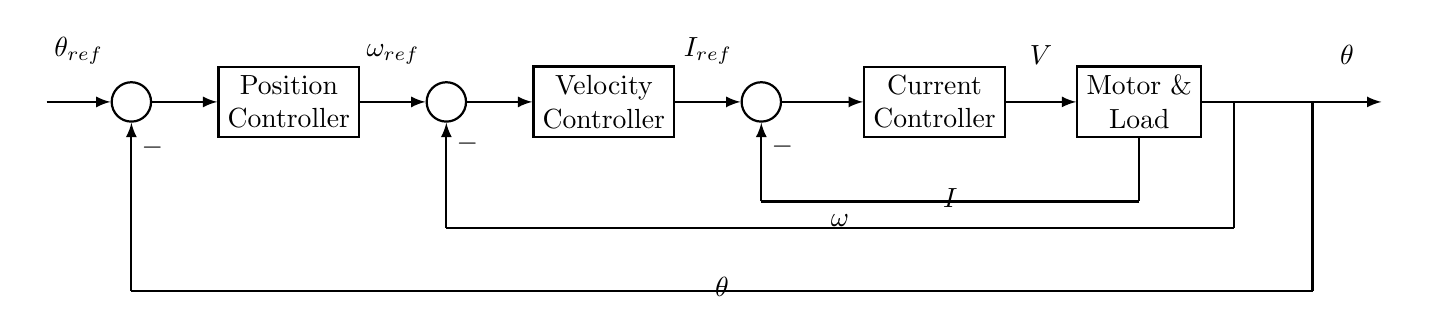
\begin{tikzpicture}[auto, >=latex]
        % تعريف الأنماط
        \tikzstyle{block} = [draw, rectangle, minimum height=2.5em, minimum width=3em, align=center, thick]
        \tikzstyle{sum} = [draw, circle, inner sep=0pt, minimum size=0.5cm, thick]
        
        \node (ref_pos) {};
        \node [sum, right of=ref_pos, node distance=1.2cm] (sum_pos) {};
        \node [block, right of=sum_pos, node distance=2cm] (ctrl_pos) {\textenglish{Position}\\\textenglish{Controller}};
        
        \node [sum, right of=ctrl_pos, node distance=2cm] (sum_vel) {};
        \node [block, right of=sum_vel, node distance=2cm] (ctrl_vel) {\textenglish{Velocity}\\\textenglish{Controller}};
        
        \node [sum, right of=ctrl_vel, node distance=2cm] (sum_cur) {};
        \node [block, right of=sum_cur, node distance=2.2cm] (ctrl_cur) {\textenglish{Current}\\\textenglish{Controller}};
        
        \node [block, right of=ctrl_cur, node distance=2.6cm] (motor) {\textenglish{Motor \&}\\\textenglish{Load}};
        
        % نقاط التفرع
        \coordinate [right of=motor, node distance=1.2cm] (takeoff_vel);
        \coordinate [right of=takeoff_vel, node distance=1cm] (takeoff_pos);
        \node [right of=takeoff_pos, node distance=1cm] (out_pos) {};

        % المسارات الأمامية مع إزاحة المتغيرات للأعلى
        \draw [->, thick] (ref_pos) -- node[midway, yshift=0.35cm] {$\theta_{ref}$} (sum_pos);
        \draw [->, thick] (sum_pos) -- (ctrl_pos);
        \draw [->, thick] (ctrl_pos) -- node[midway, yshift=0.35cm] {$\omega_{ref}$} (sum_vel);
        \draw [->, thick] (sum_vel) -- (ctrl_vel);
        \draw [->, thick] (ctrl_vel) -- node[midway, yshift=0.35cm] {$I_{ref}$} (sum_cur);
        \draw [->, thick] (sum_cur) -- (ctrl_cur);
        \draw [->, thick] (ctrl_cur) -- node[midway, yshift=0.35cm] {$V$} (motor);
        
        % خط الخرج
        \draw [-, thick] (motor) -- (takeoff_vel);
        \draw [-, thick] (takeoff_vel) -- (takeoff_pos);
        \draw [->, thick] (takeoff_pos) -- node[midway, yshift=0.35cm] {$\theta$} (out_pos);

        % التغذية الراجعة للتيار
        \draw [thick] (motor.south) -- ++(0,-0.8) coordinate (fb_I);
        \draw [thick] (fb_I) -- node[midway, yshift=0.3cm] {$I$} (fb_I -| sum_cur.south);
        \draw [->, thick] (fb_I -| sum_cur.south) -- node[pos=0.7, right] {$-$} (sum_cur.south);
        
        % التغذية الراجعة للسرعة
        \draw [thick] (takeoff_vel) -- ++(0,-1.6) coordinate (fb_w);
        \draw [thick] (fb_w) -- node[midway, yshift=0.3cm] {$\omega$} (fb_w -| sum_vel.south);
        \draw [->, thick] (fb_w -| sum_vel.south) -- node[pos=0.8, right] {$-$} (sum_vel.south);
        
        % التغذية الراجعة للموقع
        \draw [thick] (takeoff_pos) -- ++(0,-2.4) coordinate (fb_t);
        \draw [thick] (fb_t) -- node[midway, yshift=0.3cm] {$\theta$} (fb_t -| sum_pos.south);
        \draw [->, thick] (fb_t -| sum_pos.south) -- node[pos=0.85, right] {$-$} (sum_pos.south);

    \end{tikzpicture}%
    }
    \caption[المخطط الصندوقي لهيكلية حلقات التحكم المتداخلة في أنظمة السيرفو]{\centering المخطط الصندوقي لهيكلية حلقات التحكم المتداخلة في أنظمة السيرفو}
    \label{fig:cascaded_loops}
\end{figure}

\subsection{الحلقة الداخلية: حلقة التيار/العزم (\textenglish{Current/Torque Loop})}
تُعد حلقة التحكم في التيار هي خط الدفاع الأول والأسرع استجابة. تقع هذه الحلقة فعلياً داخل مشغل السيرفو (\textenglish{Servo Drive})، والهدف الأساسي منها هو التحكم الدقيق في التيار المار عبر ملفات العضو الثابت لإجبار المحرك على إنتاج العزم الميكانيكي المطلوب $T_{ref}$.

تُحكم الديناميكا الكهربائية بالمعادلة التفاضلية التالية:
$$V(t) = R \cdot i(t) + L \frac{di(t)}{dt} + E_b(t)$$
وبما أن العزم الميكانيكي يتناسب طردياً مع التيار الفعال ($T = K_t \cdot i$)، فإن التحكم في التيار يعني فعلياً التحكم في العزم. نظراً لصغر الثابت الزمني الكهربائي $\tau_e = L/R$، يُستخدم متحكم تناسبي-تكاملي (\textenglish{PI}) بترددات أخذ عينات عالية جداً تصل إلى عشرات الكيلوهرتز للتعامل مع التغيرات اللحظية وتقليل خطأ التيار إلى الصفر.

\subsection{الحلقة الوسطى: حلقة السرعة (\textenglish{Velocity Loop})}
وظيفتها الأساسية هي مقارنة السرعة المطلوبة $\omega_{ref}$ (القادمة من مخرج حلقة الموقع) مع السرعة الفعلية $\omega$ (المقاسة بواسطة المشفر)، ومن ثم توليد إشارة مرجعية للتيار $I_{ref}$ للحلقة الداخلية.

نظراً لأن الأنظمة الميكانيكية تتعرض باستمرار للاحتكاك واضطرابات التحميل الخارجية، يُستخدم بشكل شبه دائم متحكم تناسبي-تكاملي (\textenglish{PI}) في هذه الحلقة:
\begin{itemize}
    \item \textbf{الجزء التناسبي (\textenglish{P}):} يوفر استجابة فورية لأخطاء السرعة اللحظية.
    \item \textbf{الجزء التكاملي (\textenglish{I}):} يضمن القضاء التام على خطأ الحالة المستقرة عند تطبيق عزم حمل ثابت على المحرك.
\end{itemize}

\subsection{الحلقة الخارجية: حلقة الموقع (\textenglish{Position Loop})}
هي الحلقة الأبطأ من حيث سرعة الاستجابة. تستقبل مسار الحركة المطلوب $\theta_{ref}$، وتقارنه بالموقع الزاوي الفعلي $\theta$، لتُصدر السرعة المطلوبة $\omega_{ref}$ للحلقة الوسطى.

على عكس حلقة السرعة، يُكتفى عادةً باستخدام متحكم \textbf{تناسبي فقط (\textenglish{P Controller})} في حلقة الموقع. ويعود السبب الرياضي في ذلك إلى العلاقة التكاملية بين السرعة والموقع:
$$\theta(t) = \int_{0}^{t} \omega(\tau) d\tau$$
النظام الميكانيكي يمتلك بطبيعته "مُكاملاً طبيعياً" ($1/s$). لذلك، إضافة جزء تكاملي إضافي سيؤدي إلى تقليل هامش الاستقرار والتسبب باهتزاز المحرك وتجاوز الهدف (\textenglish{Overshoot}).
%\input{sections_cha3/velocity_position_loops}
\section{تحسين الاستجابة باستخدام التوقع المسبق (\textenglish{Feedforward Control})}
\label{sec:feedforward_control}

تعتمد هيكلية التحكم بالتغذية الراجعة (\textenglish{Feedback Control}) بشكل أساسي على وجود خطأ دائم (\textenglish{Error}) لتوليد إشارة التحكم. هذا يعني أن النظام سيُعاني دائماً من تأخير زمني (\textenglish{Lag}) أثناء الفترات العابرة، مثل أوقات التسارع والتباطؤ السريع، مما يقلل من دقة التتبع الديناميكي للمسار.

للتغلب على هذا القصور الجوهري، تُزود أنظمة السيرفو الحديثة بمسارات تحكم إضافية تُعرف بـ \textbf{التحكم بالتوقع المسبق (\textenglish{Feedforward Control})}. تعتمد هذه الاستراتيجية على حقن إشارات استباقية مباشرة في حلقات التحكم بناءً على المعرفة المسبقة بالمسار المطلوب والنموذج الرياضي للآلة، وذلك لتقليل العبء عن متحكمات الـ \textenglish{PID} وتقليص خطأ التتبع إلى مستويات تقترب من الصفر.

% مخطط يوضح إضافة مسارات التوقع المسبق
\begin{figure}[h!]
    \centering
    \resizebox{\textwidth}{!}{%
    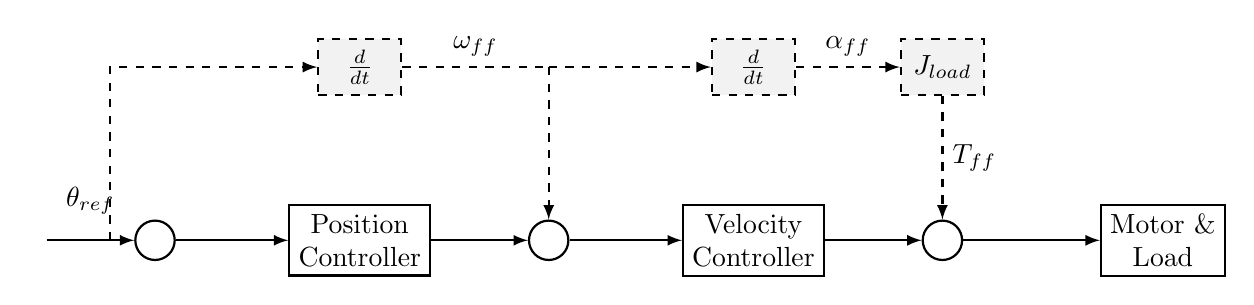
\begin{tikzpicture}[auto, >=latex]
        % تعريف الأنماط
        \tikzstyle{block} = [draw, rectangle, minimum height=2.5em, minimum width=4em, align=center, thick]
        \tikzstyle{ffblock} = [draw, rectangle, minimum height=2em, minimum width=3em, align=center, thick, fill=gray!10, dashed]
        \tikzstyle{sum} = [draw, circle, inner sep=0pt, minimum size=0.5cm, thick]
        
        % المسار الأساسي
        \node (ref_pos) {};
        \node [sum, right of=ref_pos, node distance=1.5cm] (sum_pos) {};
        \node [block, right of=sum_pos, node distance=2.6cm] (ctrl_pos) {\textenglish{Position}\\\textenglish{Controller}};
        
        \node [sum, right of=ctrl_pos, node distance=2.4cm] (sum_vel) {};
        \node [block, right of=sum_vel, node distance=2.6cm] (ctrl_vel) {\textenglish{Velocity}\\\textenglish{Controller}};
        
        \node [sum, right of=ctrl_vel, node distance=2.4cm] (sum_cur) {};
        \node [block, right of=sum_cur, node distance=2.8cm] (plant) {\textenglish{Motor \&}\\\textenglish{Load}};

        % مسارات التوقع (Feedforward) - تمت المحاذاة العمودية لمنع التداخل
        \node [ffblock, above of=ctrl_pos, node distance=2.2cm] (deriv1) {$\frac{d}{dt}$};
        \node [ffblock, above of=ctrl_vel, node distance=2.2cm] (deriv2) {$\frac{d}{dt}$};
        % وضع كتلة القصور الذاتي فوق نقطة الجمع تماماً
        \node [ffblock] at (sum_cur |- deriv2) (inertia) {$J_{load}$};

        % رسم المسارات الأساسية
        \draw [->, thick] (ref_pos) -- node[midway, yshift=0.2cm] {$\theta_{ref}$} (sum_pos);
        \draw [->, thick] (sum_pos) -- (ctrl_pos);
        \draw [->, thick] (ctrl_pos) -- (sum_vel);
        \draw [->, thick] (sum_vel) -- (ctrl_vel);
        \draw [->, thick] (ctrl_vel) -- (sum_cur);
        \draw [->, thick] (sum_cur) -- (plant);
        
        % رسم مسارات التوقع المسبق بدقة هندسية
        \coordinate (takeoff_ff) at ([xshift=0.8cm]ref_pos.east);
        \draw [->, thick, dashed] (takeoff_ff) |- (deriv1.west);
        
        % التفرع الأول (السرعة)
        \draw [thick, dashed] (deriv1.east) -- node[midway, above] {$\omega_{ff}$} (deriv1.east -| sum_vel) coordinate (drop_w);
        \draw [->, thick, dashed] (drop_w) -- (deriv2.west);
        \draw [->, thick, dashed] (drop_w) -- (sum_vel.north);
        
        % التفرع الثاني (التسارع والعزم)
        \draw [->, thick, dashed] (deriv2.east) -- node[midway, above] {$\alpha_{ff}$} (inertia.west);
        \draw [->, thick, dashed] (inertia.south) -- node[midway, right] {$T_{ff}$} (sum_cur.north);

    \end{tikzpicture}%
    }
    \caption[مخطط يوضح حقن إشارات التوقع المسبق (السرعة والعزم) في حلقات التحكم]{\centering مخطط يوضح حقن إشارات التوقع المسبق (السرعة والعزم) في حلقات التحكم الأساسية}
    \label{fig:feedforward}
\end{figure}

تُقسم إشارات التوقع المسبق في أنظمة الحركة إلى نوعين رئيسيين، كما هو موضح في المخطط (\ref{fig:feedforward}):

\subsection{توقع السرعة المسبق (\textenglish{Velocity Feedforward})}
يتم اشتقاق المسار الزاوي المطلوب $\theta_{ref}$ بالنسبة للزمن للحصول على السرعة المرجعية المطلوبة $\omega_{ff}$. تُضاف هذه الإشارة مباشرة إلى مدخل حلقة السرعة (تتجاوز متحكم الموقع). 
\begin{itemize}
    \item \textbf{الفائدة الهندسية:} يقضي هذا المسار بشكل شبه كامل على خطأ التتبع الموضعي (\textenglish{Following Error}) أثناء الحركة بسرعة ثابتة، حيث لا يضطر متحكم الموقع للانتظار حتى يتراكم الخطأ ليُصدر أمر الحركة.
\end{itemize}

\subsection{توقع العزم المسبق (\textenglish{Torque/Acceleration Feedforward})}
لتحقيق تسارع ديناميكي عالٍ دون إرهاق متحكم السرعة، يتم اشتقاق السرعة المرجعية مرة أخرى للحصول على التسارع الزاوي المطلوب $\alpha_{ff}$. بضرب هذا التسارع في عزم القصور الذاتي الكلي للنظام ($J_{load}$)، نحصل على العزم الديناميكي المطلوب $T_{ff}$ بناءً على قانون نيوتن الثاني:
$$T_{ff} = J_{load} \cdot \alpha_{ff}$$
تُضاف هذه الإشارة مباشرة إلى مدخل حلقة التيار.
\begin{itemize}
    \item \textbf{الفائدة الهندسية:} يوفر هذا المسار العزم الإضافي اللازم للتغلب على القصور الذاتي اللحظي أثناء التسارع والتباطؤ، مما يمنع انخفاض سرعة المحرك تحت تأثير الحمل، ويجعل استجابة النظام تبدو وكأنها لا تمتلك قصوراً ذاتياً.
\end{itemize}

\textbf{ملاحظة جوهرية في نظرية التحكم:} على عكس زيادة مكاسب (\textenglish{Gains}) متحكمات الـ \textenglish{PID} التي قد تؤدي إلى عدم استقرار النظام أو الرنين الميكانيكي، فإن إضافة مسارات التوقع المسبق (\textenglish{Feedforward}) \textbf{لا تؤثر إطلاقاً على استقرار حلقة التحكم المغلقة}، لأنها تُحقن من خارج حلقة التغذية الراجعة، مما يجعلها أداة قوية جداً وآمنة لتحسين الأداء الديناميكي.